%% Preamble
  \documentclass{homework}

  \hwTitle{Assignment\ \#3 - Electro-statics} % Assignment title
  \hwDueDate{Friday,\ May\ 24,\ 2013} % Due date
  \hwClass{Physics\ 441} % Course/class
  % \hwInstructor{Manuel Berrondo} % Teacher/lecturer
  \hwAuthor{Spencer Lyon} % Your name

  \usepackage{setspace}

  %% Added by Spencer for source code highlighting
  \usepackage{listings}
  \usepackage{color}

  \definecolor{dkgreen}{rgb}{0,0.6,0}
  \definecolor{gray}{rgb}{0.5,0.5,0.5}
  \definecolor{mauve}{rgb}{0.58,0,0.82}

  \lstset{frame=tb,
    language=Python,
    aboveskip=3mm,
    belowskip=3mm,
    showstringspaces=false,
    columns=flexible,
    basicstyle={\small\ttfamily},
    numbers=left,
    stepnumber=5,
    numberstyle=\tiny\color{gray},
    keywordstyle=\color{blue},
    commentstyle=\color{dkgreen},
    stringstyle=\color{mauve},
    breaklines=true,
    breakatwhitespace=true
    tabsize=4
  }

% New commands I use a lot
  \newcommand\ve{\varepsilon}
  \newcommand{\bs}[1]{\ensuremath{\boldsymbol{#1}}}
  \newcommand{\bhat}[1]{\ensuremath{\boldsymbol{\hat{#1}}}}
  \newcommand{\cross}[2]{\ensuremath{\boldsymbol{#1} \times \boldsymbol{#2}}}
  \newcommand{\curl}[1]{\ensuremath{\cross{\nabla}{\bs{#1}}}}
  \newcommand{\diver}[1]{\ensuremath{\nabla \times \bs{#1}}}

  % partial derivative as a fraction
  \newcommand{\fracpd}[2]{
    \ensuremath{\frac{\partial #1}{\partial #2}}
  }

  % fraction with parenthesis around it
  \newcommand{\pfrac}[2]{
    \ensuremath{ \left( \frac{#1}{#2} \right)}
  }

  % Just a vector in xhat yhat zhat
   \newcommand{\xyzvec}[3]{
   \ensuremath{
      (#1) \bhat{x} + (#2) \bhat{y} + (#3) \bhat{z}
   }
   }

  % Express integral bounds in parenthesis with tall vertical bar
   \newcommand{\intbounds}[3]{
   \ensuremath{
      \left. \left( #1 \right) \right|_{#2}^{#3}
   }
   }

\begin{document}

\maketitle

\begin{homeworkProblem}[Problem 2.6]

  Find the electric field a distance $z$ above the center of a circular loop of radius $r$ that carries a uniform line charge $\lambda$

  \vspace{.2in}

  \problemAnswer{ % Answer

    We will be using the following two equations
    $$ \bs{E}(\bs{r})_{\text{line}} = \frac{1}{4 \pi \ve_0} \int \frac{\lambda(\bs{r}')}{r^2} \bhat{r} da' $$
    $$ \bs{E}(\bs{r})_{\text{surf}} = \frac{1}{4 \pi \ve_0} \int \frac{\sigma(\bs{r}')}{r^2} \bhat{r} da' $$

    The easiest way to do this problem is to break the disk up into a series of circular rings, each with a radius $r$. We see that $\bs{r}'$ can be found using the Pythagorean theorem: $\bs{r}' = \sqrt{\bs{r}^2 + z^2} \cos \theta \bhat{z}$, where $\cos \theta = \frac{z}{r}$. Using symmetry we can say that $dl = 2 \pi $Putting all this together we can get the electric field for each ring is

    \begin{align*}
      E_{ring} &= \frac{1}{4 \pi \ve_0} \int \frac{\lambda(\bs{r}')}{r^2} \bhat{r} d l \\
        &= \frac{1}{4 \pi \ve_0} \int \frac{\lambda(\bs{r}') z}{(r^2 + z^2)^{3/2}} \bhat{z} dl \\
        &= \frac{1}{4 \pi \ve_0} \frac{2 \pi r z \lambda(\bs{r}')}{(r^2 + z^2)^{3/2}} \bhat{z}
    \end{align*}

    We are given that the charge is a uniform $\sigma$, so $\lambda(\bs{r}') = \sigma dr$. Ready to plug that in and integrate from $0$ to $R$ (Note I let the computer do the actual integral for me).

    \begin{align*}
      E_{ring} &= \int_0^R \frac{1}{4 \pi \ve_0} \frac{2 \pi r z \lambda(\bs{r}')}{(r^2 + z^2)^{3/2}} \bhat{z} \\
        &= \frac{\sigma z}{2 \ve_0} \int_0^R \frac{r}{(r^2 + z^2) ^{3/2}} dr \\
        &= \frac{\sigma z}{2 \ve_0} \left[\frac{1}{z} - \frac{1}{\sqrt{R^2  + z^2}} \right] \bhat{z}
    \end{align*}

    In the limit as $R \rightarrow \infty$ the second term goes to zero and we get $E = \frac{\sigma}{2 \ve_0} \bhat{z}$

    When $z >> R$ we need to expand the square root in the denominator. $\frac{1}{\sqrt{R^2 + z^2}} = 1/z \left( 1 + \frac{R^2}{z^2}\right) \approx 1/z \left(1 - \frac{R^2}{2z^2} \right) \approx \frac{R^2}{2z^3}$ so we can say that $E = \frac{\sigma R^2}{4 \ve_0 z^2} $ \qed

  }
\end{homeworkProblem}

\begin{homeworkProblem}[Problem 2.10]

  A charge $q$ site at the back corner of a cube. What is the flux of $\bs{E}$ through a side not touching that corner?

  \vspace{.2in}

  \problemAnswer{ % Answer

    We will be using Gauss' law. To do that we need to think of a convenient gaussian surface such that we can use symmetry arguments to make this problem easier. One such surface is a larger cube that puts the charge at the very center. We can then think of our original surface as being one of 4 panels on a side of the larger cube. This "pabel" is one of 24 similar panels that evenly share the total flux caused by our point charge. It is then simple to say $$\text{flux}_{\text{panel}} = \frac{q}{24 \ve_0}$$ \qed

  }
\end{homeworkProblem}

\begin{homeworkProblem}[Problem 2.16]

  A long coaxial cable carries a uniform volume charge density $\rho$ on the inner cylinder (radius $a$), and a uniform surface charge density on the outer cylindrical shell (radius $b$).  This surface charge is negative and is of just the right magnitude that the cable as a whole is electrically neutral. Find the electric field in each of the three regions:

  \begin{enumerate}
    \item inside the inner cylinder ($s < a$)
    \item Between the cylinders ($a < s < b$)
    \item Outside the cable ($s < b$)
  \end{enumerate}

  Plot $|\bs{E}|$ as a function of $s$.

  \vspace{.2in}

  \problemAnswer{ % Answer

  \begin{enumerate}
    \item For the first part we will take as a Gaussian surface a cylinder of radius a. We will be using $\oint \bs{E} \cdot d\bs{a}$, but due to symmetry simplifies down to $E \oint d \bs{a} = E 2 \pi s l$. We now apply Gauss' Law and say that this must be equal to $\frac{Q}{\ve_0}$. Doing so we can get an expression and solve for E

      \begin{align*}
        2 E \pi s l &= \frac{Q}{\ve_0} \\
        2E \pi s l &= \frac{\rho \pi s^2 l } {\ve_0}\\
        E &= \frac{\rho s}{2 \ve_0}
      \end{align*}

      This points radially outward in he $\bhat{s}$ direction.
    \item For the second part we choose as Gaussian surface a cylinder of radius $s$, where $a< s <b$.In this case we end up with the exact same expressions, except $Q = \rho \pi a^2 l $ (sub $a$ for $s$, because when $ s>a$ no additional charge is enclosed). This allows us to substitute $a$ for $s$ in the final part and get that $$ E = \frac{\rho a^2}{2 s \ve_0} \bhat{s}$$

    \item Finally for the third part we recognize that anywhere on or beyond the surface of the outer cylinder has a neutral charge, therefore $$E=0$$
  \end{enumerate}

  In Figure ~\ref{fig:216} I have plotted the magnitude of the electric field. Below is the code used to make the plot.

  \setstretch{0.6}
  \lstinputlisting[language=Python, firstline=1, lastline=49]{hw3.py}
  \setstretch{1.5}

  \qed
  }


  \begin{figure}[!h]
    \begin{centering}
    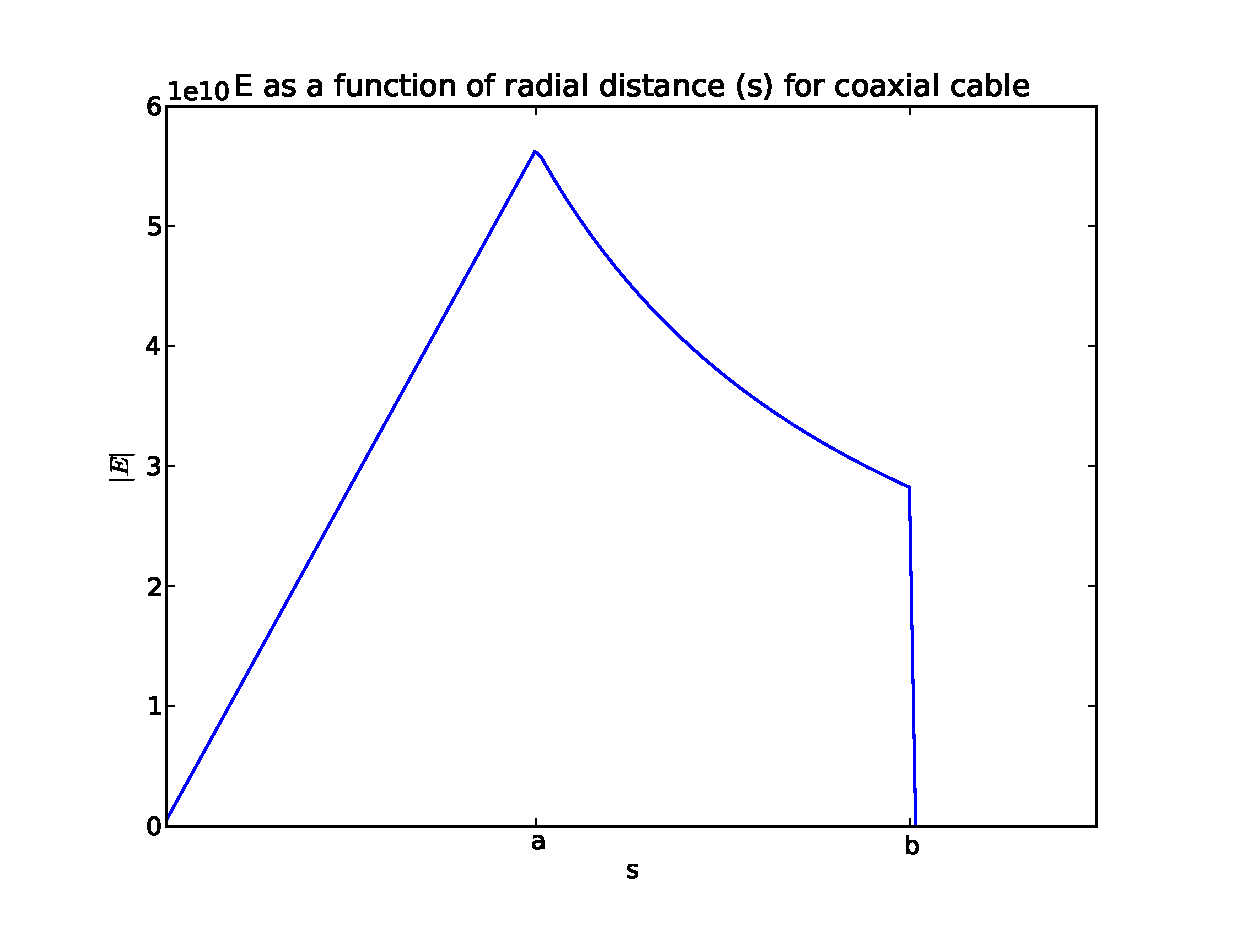
\includegraphics[width=4.5in, height=3in]{E2_16.eps}
    \caption{The magnitude of the electric field for the coaxial cable in problem 2.16}
    \label{fig:216}
    \end{centering}
  \end{figure}
\end{homeworkProblem}

\begin{homeworkProblem}[Problem 2.24]

  For the configuration of problem 2.16, find the potential difference between a point on the axis and a point on the outer cylinder. Note that it its not necessary to commit yourself to a particular reference point if you use

  \begin{align*}
    V(\bs{b}) - V(\bs{a}) &= - \int_{\mathbb{O}}^{\bs{b}} \bs{E} \cdot d \bs{l} + \int_{\mathbb{O}}^{\bs{a}} \bs{E} \cdot d \bs{l} \\
      &= - \int_{\mathbb{O}}^{\bs{b}} \bs{E} \cdot d \bs{l} - \int_{\bs{a}}^{\mathbb{O}} \bs{E} \cdot d \bs{l} \\
      &= - \int_{\bs{a}}^{\bs{b}} \bs{E} \cdot d \bs{l}
  \end{align*}

  \vspace{.2in}

  \problemAnswer{ % Answer

  For the point on the cylinder $s=b$ and for the point on the axis $s=0$. We now need to integrate from $0 \rightarrow b$. As we learned in previous problem, the field changes so we will break the integral up into into two integrals going from $0 \rightarrow a$ and $a \rightarrow b$. I show this below.

  \begin{align*}
    - \int_0^b \bs{E} \cdot d \bs{a} &= -\left (\int_0^a \bs{E} \cdot d \bs{a} + \int_a^b \bs{E} \cdot d \bs{a} \right) \\
      &= - \left(\int_0^a E ds + \int_a^b E ds \right) \\
      &= - \left(\frac{\rho}{2 \ve_0 }\int_0^a s ds  +  \frac{\rho a^2}{2 \ve_0}  \int_a^b \frac{1}{s} ds \right) \\
      &= - \left( \frac{\rho}{2 \ve_ 0} \left.  \frac{s^2}{2} \right|_0^a  +  \left.  \frac{\rho a^2}{2 \ve_0} \ln s \right|_a^b\right) \\
      &= - \frac{\rho a^2}{2 \ve_0}  \left(\frac{b}{a}+ \ln\left(\frac{b}{a}\right) \right)
  \end{align*}

  \qed
  }
\end{homeworkProblem}

\begin{homeworkProblem}[Problem 2.29]

  Check that $$V(\bs{r}) = \frac{1}{4 \pi \ve_0} \int \frac{\rho(\bs{r}')}{r} d \tau '$$ satisfies Poisson's equation, by applying the Laplacian and using $$\nabla^2 \frac{1}{r} = -4 \pi \delta^3(\bs{r})$$

  \vspace{.2in}

  \problemAnswer{ % Answer

  Poisson's equation is $$\nabla^2 \phi = f $$ We want to show that $\nabla^2 V$ ends up being a scalar function in $r$. We do this below. Note that we apply the hint given about the Laplacian of $\frac{1}{r}$

  \begin{align*}
    \nabla^2 V &= \frac{1}{4 \pi \ve_0} \nabla^2 \int\frac{\rho(\bs{r}')}{r} d \tau' \\
      &= \frac{1}{4\pi\ve_0} \int \rho(\bs{r}') \nabla^2 \pfrac{1}{r} d \tau' \\
      &= \frac{1}{4\pi\ve_0} \int \rho(\bs{r}') \left[-4 \pi \delta^3(\bs{r} - \bs{r}') \right] d \tau' \\
      &= - \frac{\rho(\bs{r})}{\ve_0}
  \end{align*}

  I made the last simlification by canceling out the $4\pi$ in the numerator and denominator and using identities for integrals of products, where one of the things being multiplied is a delta function.
  \qed

  }
\end{homeworkProblem}

\begin{homeworkProblem}[Problem 2.38]

  A metal sphere of radius $R$, carrying charge $q$, is surrounded by a thick concentric metal shell (inner radius $a$, outer radius $b$). The shell carries no net charge.

  \begin{enumerate}
    \item Find the surface charge density $\sigma$ at $R$, $a$, and $b$.
    \item Find the potential at the center, using infinity as a reference point
    \item Now the outer surface is touched to a grounding wire, which drains off charge and lowers its potential to zero (same as infinity). How do your answers to the previous parts change?
  \end{enumerate}

  \vspace{.2in}

  \problemAnswer{ % Answer

    \begin{enumerate}
      \item Equation 2.10 in the book says $$\bs{E}(\bs{r}) = \frac{1}{4 \pi \ve_0} \frac{q}{r^2} \bhat{r} $$ Then equation 2.48 says $$\bs{E} = \frac{\sigma}{\ve_0} \bhat{n}$$ Putting these equations together we see that $$\sigma  = \frac{q}{4 \pi r^2} \bhat{n}$$ We will apply this expression to the three cases
        \begin{itemize}
          \item at $R$: $r = R$ and $\bhat{n}= 1$ so $\sigma = \frac{q}{4 \pi R^2} $
          \item at $a$: $r = a$ and $\bhat{n}= -1$ so $\sigma = - \frac{q}{4 \pi a^2} $. Note that it is negative at this time because it is pointing into the middle layer of the shell, not outside.
          \item at $b$: $r = b$ and $\bhat{n}= 1$ so $\sigma =  \frac{q}{4 \pi b^2} $
        \end{itemize}
    \item We will need to integrate $\bs{E} \cdot d \bs{l} = \frac{1}{4 \pi \ve_0} \frac{q}{r^2} dr$ from $-\infty$ to $0$. To do this we will break the integral up into the following integrals: $[-\infty, b], [b, a], [a, R] , [R, 0]$. From the problem description we know that $\bs{E} = 0$ inside the inner radius $R$ (interval $[R, 0]$) and in between the shell (interval $[b, a]$).
      \begin{align*}
        V(0) &= - \int_{-\infty}^0 \bs{E} \cdot d \bs{l} \\
          &= - \int_{-\infty}^0 \frac{1}{4 \pi \ve_0} \frac{q}{r^2} dr\\
          &= -\left( \int_{-\infty}^b  \frac{1}{4 \pi \ve_0} \frac{q}{r^2} dr + \int_b^a 0 dr+ \int_a^R  \frac{1}{4 \pi \ve_0} \frac{q}{r^2} dr+ \int_R^0 0 dr\right) \\
          &= - \left(\intbounds{- \frac{q}{4 \ve_0 \pi r}}{-\infty}{b}  + 0 + \intbounds{- \frac{q}{4 \ve_0 \pi r}}{a}{R} + 0\right)\\
          &= - \left(- \frac{q}{4 b \ve_0 \pi} + \frac{q}{4 a \ve_0 \pi} - \frac{q}{4 R \ve_0 \pi} \right) \\
          &= \frac{1}{4 \pi \ve_0} \left( \frac{q}{b} + \frac{q}{R} - \frac{q}{a}\right)
      \end{align*}
    \item It is easy to answer this part qualitatively. For part a, If the outer surface  at $r=b$ is grounded, $E=0$ there which means that $\sigma = 0 $ there. For part b, we just have no contribution from the electric field at b so the answer would be $\frac{1}{4 \pi \ve_0} \left(\frac{q}{R} - \frac{q}{a}\right)$.
    \end{enumerate}
    \qed
  }
\end{homeworkProblem}

\begin{homeworkProblem}[Problem 2.43]

  Find the capacitance per unit length of two coaxial metal cylindrical tubes of radii $a$ and $b$.

  \vspace{.2in}

  \problemAnswer{ % Answer

    We looked at coaxial cables in problems 2.16 and 2.24. In those problems we allied Gauss' law and derived the expression $ E 2 \pi s L = \frac{Q}{\ve_0}$ which leads us to $$\bs{E} = \frac{Q}{2 \pi \ve_0 L} \frac{1}{s} \bhat{s}$$. If we apply this to our problem and we say that the charge on the inner cable is $Q$ we can get an expression for V.

    \begin{align*}
      V(b) - V(a) &= - \int_a^b \bs{E} \cdot d \bs{l} \\
        &= - \int_a^b \frac{Q}{2 \pi \ve_0 L} \frac{1}{s} \bhat{s} \cdot d \bs{l} \\
        &= -  \frac{Q}{2 \pi \ve_0 L} \int_a^b \frac{1}{s} ds \\
        &= -  \frac{Q}{2 \pi \ve_0 L} \ln \pfrac{b}{a}
    \end{align*}

    The way we have set this problem up $V = V(a) - V(b) = - (V(b) - V(a)) =  \frac{Q}{2 \pi \ve_0 L} \ln \pfrac{b}{a} $. We can now apply the identity for capacitance and divide by length to get capacitance per unit length:

    \begin{align*}
      \frac{C}{L} &= \pfrac{Q}{V} \frac{1}{L} \\
        &= \pfrac{Q}{ \frac{Q}{2 \pi \ve_0 L} \ln \pfrac{b}{a}} \frac{1}{L} \\
        &= \frac{2 \pi \ve_0}{\ln \pfrac{b}{a}}
    \end{align*}
    \qed

  }
\end{homeworkProblem}

\begin{homeworkProblem}[Problem 2.50]

  The electric potential of some configuration is given by the expression $$ V(\bs{r}) = A \frac{e^{-\lambda r}}{r}$$ where $A$ and $\lambda$ are constants. Find the electric field $\bs{E}(\bs{R})$, the charge density $\rho(r)$, and the total charge $Q$. [Answer: $\rho=\ve_0 A (4 \pi \delta^3 (\bs{r}) - \lambda^2 e^{-\lambda r} / r$]

  \vspace{.2in}

  \problemAnswer{ % Answer

    We know that $E = - \nabla V$. We use this identity to solve for the electric field.

    \begin{align*}
      \bs{E} &= - \nabla V \\
        &= - A \left( \fracpd{}{r} \frac{e^{-\lambda r}}{r} \bhat{r}\right) \\
        &= -A \left( - \frac{\lambda e^{- \lambda r}}{r} - \frac{e^{- \lambda r}}{r^{2}} \right) \\
        &= A e^{-\lambda r} \left(\frac{\lambda}{r} + \frac{1}{r^2} \right) \bhat{r}
    \end{align*}

    Equation 2.14 gives us an expression for $\rho$ in terms of \bs{E}: $$\nabla \cdot \bs{E} = \frac{1}{\ve_0} \rho $$
    which we will apply to solve for $\rho$. Before doing do a little algebra on \bs{E} to make it in a more friendly form: $\bs{E} = A(1 + \lambda r) e^{\lambda r} \frac{\bhat{r}}{r^2}$. We will also apply the equation 1.102 to get $\nabla \cdot \frac{\bhat{r}}{r^2}$.

    \begin{align*}
      \rho &= \ve_0 \nabla \cdot \bs{E} \\
        &= \ve_0 \nabla \cdot \left( A(1 + \lambda r) e^{\lambda r} \frac{\bhat{r}}{r^2} \right) \\
        &= A \ve_0 \left( (1 + \lambda r) e^{\lambda r} \nabla \cdot \frac{\bhat{r}}{r^2} + \frac{\bhat{r}}{r^2} \cdot \nabla \left((1 + \lambda r) e^{\lambda r} \right)\right) \\
        &=A \ve_0 \left( (1 + \lambda r) e^{\lambda r} 4 \pi \delta^3(\bs{r}) + \frac{\bhat{r}}{r^2} \left[-\lambda^2 r e ^{-\lambda r} \right] \right) \\
        &= A \ve_0  \left(4 \pi \delta^3 (\bs{r}) - \frac{\lambda^2}{r} e^{-\lambda r} \right)
      \end{align*}

    We now solve for $Q$ using the identity that $Q = \int \rho d \tau$.

    \begin{align*}
      Q &= \int \rho d \tau \\
        &= \int A \ve_0  \left(4 \pi \delta^3 (\bs{r}) - \frac{\lambda^2}{r} e^{-\lambda r} \right) 4 \pi dr \\
        &= A \ve_0 \left[ 4 \pi \int\delta^3(r) d \tau - 4 \pi \lambda^2 \int \frac{e^{-\lambda r}}{r} dr \right] \\
        & = A \ve_0 \left(4 \pi  - 4 \pi \lambda^2 \int_0^{\infty} r e ^{-\lambda r} dr \right) \\
        &= A \ve_0 \left(4 \pi  -  4 \pi\lambda^2 / \lambda^2 \right) \\
        &= 0
    \end{align*}
    \qed
  }
\end{homeworkProblem}

\end{document}

